\chapter{Koncepció}
\label{chap:Concept}

Az évek alatt sok olyan játékkal játszottam, amelyek mélyen kidolgozott mozgásrendszerekre épülnek. Ilyen műfajok például a Movement-Shooter, bizonyos Sport játékok többnyire azok, amik gördeszkákra, görkorcsolyákra és a hasonlókra épülnek. Fontosnak tartottam itt megemlíteni a Movement-Shooter műfajt, mivel az ebbe tartozó játékok szerettették meg igazán velem a szofisztikált mozgásrendszereket és belőlük tanultam sokat. Ezen játékok tökéletesen összehangolják a finom mozdulatokat az aréna-lövöldék (mint például a Quake) gyors döntéshozatalával. Ezeket a műfajok csupán motivációként hoztam fel, ha esetleg a kedves olvasónak megjönne a kedve jobban belemenni a gyorsabb videójátékok világába.

\section{Játékmenet}

A játékmenet nem komplikált, mivel ez túlmutatna a projekt lényegén. A játékos képes mozogni minden irányba (jobb, bal, előre, hátra, és átlósan), képes ugrani, valamint a levegőben mozogni. Ez kombinálva a játékos képességé\-vel, hogy végigcsússzon az azokra kijelölt felületeken egy elég egyszerű, de erős alapot ad egy tényleges nagyobb játék elkészítéséhez. Mindezek ellenére, úgy érzem, hogy le kell szögeznem, hogy a színtér maga csupán arra szolgálna, hogy be tudjam mutatni a mozgásrendszert és vizualizálni tudjam az állapotgé\-pet munka közben. Az állapotgépet úgy terveztem meg, hogy akármilyen projektben, amely a Godot játékmotoron belül készült, használható legyen, de a logikát más játékmotorokra is ki lehet terjeszteni. A mozgásrendszerem a Tony Hawk's Proskater játéksorozatot és Bomb Rush Cyberfunk / Jet Set Radio játékmenetét vette alapul. Azzal az eltéréssel, hogy a saját projektemben megnyerési pont nincs, mivel ez túlmutatott a projektnek megszabott feladaton.

\section{Használt technológiák}
\label{subsec:UsedTech}

A használt technológiákat két részre osztanám fel: \textbf{szoftver} és \textbf{hardver}. 

\textbf{Szoftver szempontjából:}
\begin{itemize}
	\item \href{https://www.blender.org/download/}{\underline{Blender}-t} \cite{Blender} használtam a 3Ds modellek elkészítéséhez.
	\item \href{https://krita.org/en/}{\underline{Krita}-t} \cite{Krita} használtam a modellek textúráinak megrajzolásához.
	\item A diagramok megszerkesztéséhez \href{https://www.drawio.com/}{\underline{Draw.io-t}} \cite{Draw.io} használtam.
	\item A verziókövetéshez Git-et használtam.
\end{itemize}

\textbf{Hardver szempontjából a szoftvert két különböző rendszeren teszteltem és fejlesztettem:}
\begin{itemize}
	\item Asztali Számítógép:
	      \begin{itemize}
		      \item Windows 10
		      \item Processzor: AMD Ryzen 5 7600X 6-Core
		      \item AMD Radeon RX 6600
		      \item Memória (RAM): 32GB
	      \end{itemize}
	\item LENOVO IdeaPad Slim 3 15AMN8 (Laptop):
	      \begin{itemize}
		      \item Kubuntu 25.10
		      \item Processzor: 8 x AMD Ryzen 5 7520U with Radeon Graphics
		      \item Videókártya: AMD Radeon 610M
		      \item Memória (RAM): 16GB
	      \end{itemize}
\end{itemize}

Megjegyezném, hogy ez nem jelenti azt, hogy csak ezen gépigényeket elérő rendszereken működne a program, egyszerűen csak ezeken tudtam kipróbálni.
A digitális koncepció rajzok elkészítéséhez és a textúrák megalkotásá\-hoz az: XP-Pen Deco 02-őt használtam.

\section[Fejlesztési Környezet]{Fejlesztési környezet választása}
A fejlesztési környezet választásakor több szempontot is figyelembe kellett vennem:
\begin{itemize}
	\item \underline{Elérhetőség:} Mivel a fejlesztést két különböző rendszeren, két különböző operációs rendszer alatt végeztem fontos volt számomra, hogy a fejlesztési környezet elérhető legyen mind a két operációs rendszeren.
	\item \underline{Programozási Nyelv Támogatása:} Fontos szempont volt a játékmotor kiválasztásakor a C\# nyelv támogatása. Mivel a C\# nyelvet gyakran használják videójátékok programozásánál, fontosnak tartottam, hogy a szakdolgozatomat egy olyan környezetben készítsem el, ami támogatja. Nem csak a nyelv miatt, de ha sikerül elsajátítani, vagy legalább megismerkedni egy hasznos játékmotorral, az sokat segíthet majd nekem a jövőben.\\
	\begin{tabularx}{\textwidth}{
  | >{\raggedright\arraybackslash}X
  | >{\raggedright\arraybackslash}X
  | >{\raggedright\arraybackslash}X
  | >{\raggedright\arraybackslash}X | }
	\hline
	Szempont & Godot & Unity & Unreal Engine\\
	\hline
	Tanulási görbe & alacsony/közepes & közepes & magas\\
	C\# támogatás & van & natív jellegű & csak pluginnal\\
	Mozgásrendszer prototipizálás & alkalmas & alkalmas & túl nagy eszközkészlet\\
	Licensz & nyílt forráskódú & üzleti feltételekhez kötött & üzleti feltételekhez kötött\\
	Projektmérethez illeszkedés & megfelel & jó & nem alkalmas\\
	\hline
	\end{tabularx}
\end{itemize}

\section{Játékmotor, programozási nyelv és fejlesztőkörnyezet}

A játékmotor, programozási nyelv és fejlesztőkörnyezet megválasztása során fontos volt számomra a platformfüggetlenség, kompatibilitás és a hordozhatóság.
\begin{itemize}
	\item \underline{Kompatibilitás / Platformfüggetlenség:} Mivel a szoftvert két különböző operációs rendszeren fejlesztettem ezért elengedhetetlen volt az, hogy az összes projektfejlesztéshez használt program elérhető legyen mind egy Linux környezet, mind egy Windows környezet alatt. A játékmotorok, amik mindig szóba jönnek az a Unity és az Unreal Engine, viszont ezeknél az motoroknál a licensz kérdése is szóba jön. Nem egy utolsó szempont az se, hogy ezzel a rendszerrel én majd a jövőben tovább dolgozhassak akármilyen fennakadás vagy hátráltatás nélkül.
	\item \underline{Tapasztalat:} Fontos volt a meglévő tapasztalat a választott technológiával, hogy a lehető legjobbat ki tudjam hozni a projektből reális időn belül. Egy új rendszer vagy programozási nyelv megtanulása időt vett volna el, amit fejlesztésre tudtam volna használni.
\end{itemize}

\textbf{Így mindezeket a szempontokat összevetve a választásaim végül a: Godot motorra, C\# programozási nyelvre és a Visual Studio Code fejlesztőkörnyezetre esett.}

\section{Vizuális világ megtervezése}

A vizuális világ, amint már említettem a Shibuya punk esztétikára alapszik. Agresszív vonalak, elmosott, neon színek erőteljes használata és dinamikus kompozíciók definiálják, ahogyan az a \ref{JSR_Logo} ábrán is látható. Műfajalkotó játéknak számít a Jet Set Radio (amire mostantól \textbf{JSR}-ként fogok hivatkozni).

\begin{figure}[H]
	\centering
	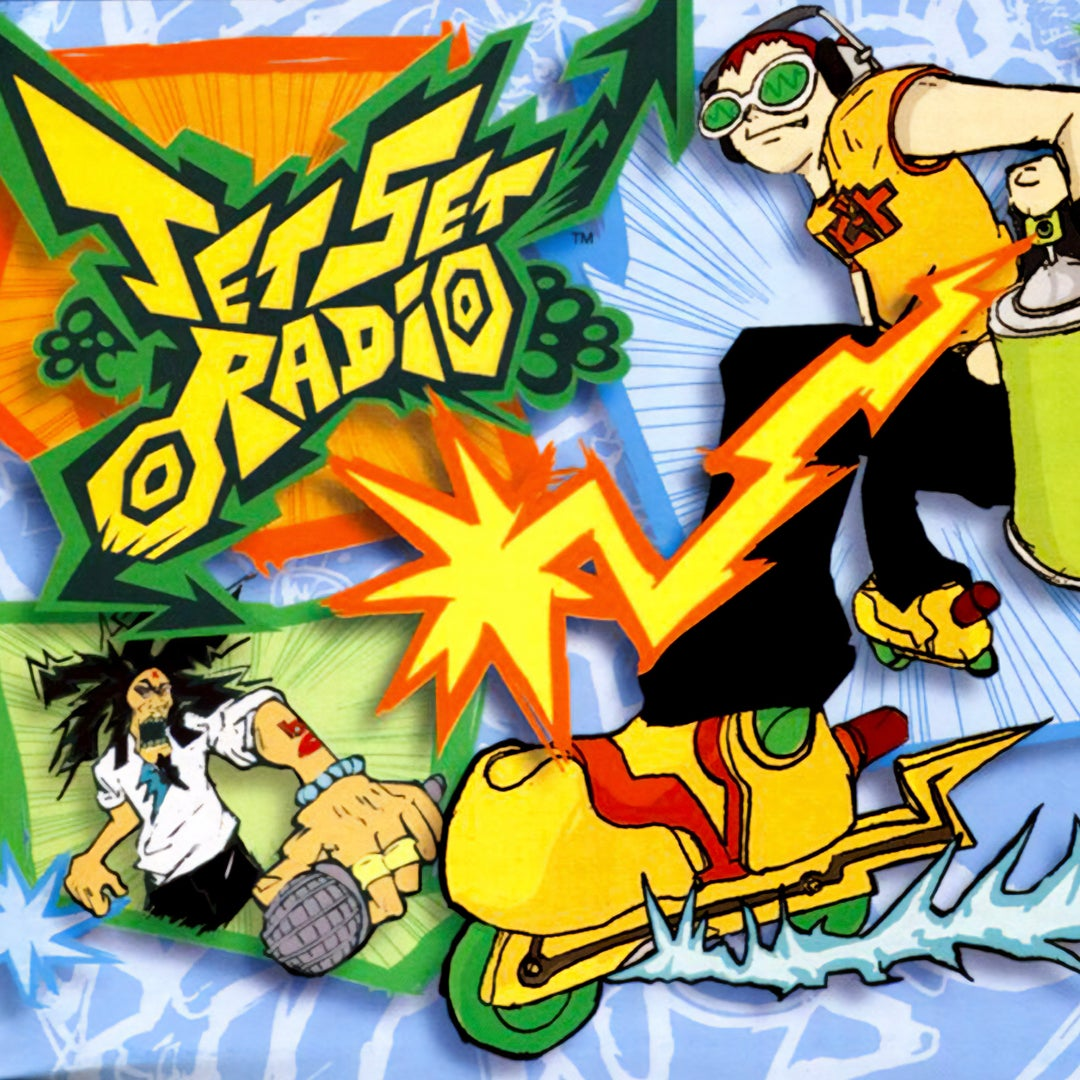
\includegraphics[height=1080px/4, width=1080px/4]{Images/JetSetRadio_Logo.jpg}
	\caption{Demonstráció az agresszív vonalakra}
	\label{JSR_Logo}
\end{figure}

A JSR 2000-ben jött ki a DreamCast konzolra. És korszakalkotó volt a játék vizuális világa, játékmenete és mozgásrendszere. Százezreket fogott meg, sajnos évekre rá sem jött ki olyan játék, ami el tudta volna csípni, hogy mi is tette a játékot annyira ikonikussá.
A játékmenetében is megtartja a dinamikusságot és az agresszív vonalakat, ami a játékosban azt az érzést kelti, hogy gyorsabb és pontosabb mint valójában, lásd azt a \ref{JSR_Thumbnail} ábrán.

\begin{figure}[H]
	\centering
	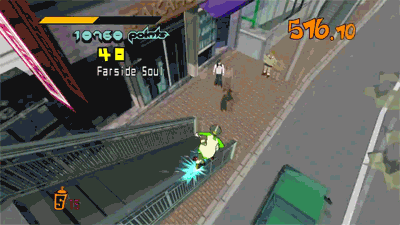
\includegraphics[width=\linewidth]{Images/JSR_Gameplay/JetSetRadio_Gameplay-2.png}
	\caption{Képpillanat a JSR játékmenetéről}
	\label{JSR_Thumbnail}
\end{figure}

Ahhoz, hogy pontosan replikálni tudjam ezeket a tulajdonságokat mélyen bele kellett magam ásnom a játék világába, de mivel egy eléggé régi játékról van szó, nem könnyen hozzáférhető. Szerencsére erre a problémára megoldást találtam egy 2023-mas ún. "Szerelmi Vallomásban" (Love Letter), a \href{https://store.steampowered.com/app/1353230/Bomb_Rush_Cyberfunk/}{Bomb Rush Cyberfunk}-ban (amire mostantól \textbf{BRCF}-ként fogok hivatkozni). A hasonlóságokat a \ref{BRCF_Logo} ábra jól mutatja.

\begin{figure}[H]
	\centering
	
\includegraphics[width=\linewidth]{Images/BombRushCyberfunk_Logo.jpg}
	\caption{Reklámkép a Bomb Rush Cyberfunk-ról}
	\label{BRCF_Logo}
\end{figure}

A játék teljes mértékben a JSR-t veszi alapul és megpróbálja replikálni a játékot annyira, amennyire csak tudja, miközben újít és iterál a meglévő koncepciókon. A játékmenet kifinomultabb, mint a JSR-nak, de képes megtartani azt az érzést, amit annak idején az elődje keltet. A \ref{BRCF_InAction} ábra is átadja ezt az érzést. A Team Reptile leírása alapján: "Dion Koster elmevilágában, ahol saját-stílusú bandák személyi jetpack-ekkel vannak felruházva, a graffiti művészet új magaslatokba szárnyal. Vágj bele te is a világba és táncolj, fess, trükköz, verd vissza a korrupt rendőrséget és foglald el a város minden zegét-zugát egy alternatív jövőben, amit életre kelt Hideki Naganuma zenéje" \cite{reptile2020}.

\begin{figure}[H]
	\centering
	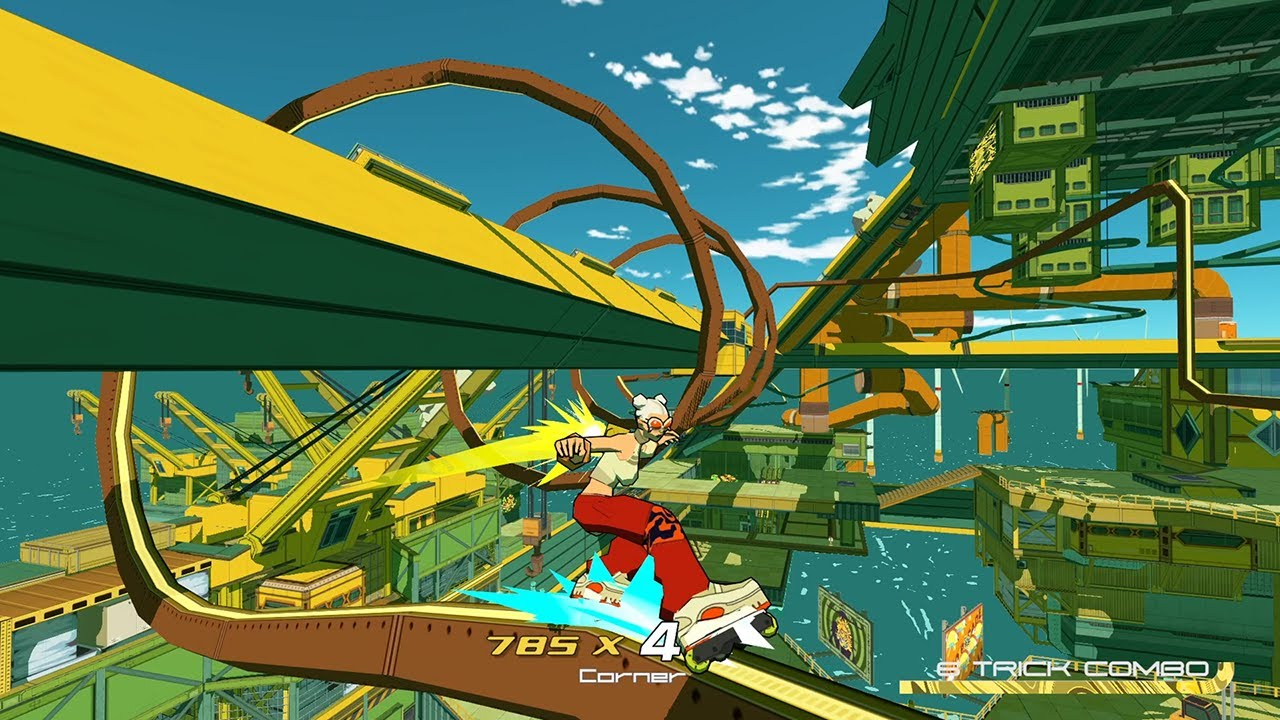
\includegraphics[width=\linewidth]{Images/BombRushCyberfunk_InAction.jpg}
	\caption{Játékbeli kép a Bomb Rush Cyberfunk-ról}
	\label{BRCF_InAction}
\end{figure}

Látszatra a két játék ugyanazt a stílust tartja, azzal a különbséggel, hogy míg a JSR egy földhöz-ragadtabb játékmenetet és világot ad át, mint ha egy, a 20-as éveiben lévő lázadó punk tini lennél, addig a BRCF egy sokkal sci-fi-sebb világba dob minket, ahol mindenkinek lehet egy jetpack a hátán, ami eszméletlen sebességekre gyorsít fel minket és rásegít a trükkjeinkre
A vizuális világ megtervezésében tehát ezeket a szempontokat vettem alapul és ezek szerint alakítottam a világot és a karaktert.


\section[Mozgásrendszer]{Mozgásrendszer megtervezése}

Most, hogy a vizuális világ megbeszélésre került, ideje áttérni arra, ami igazán fontos: a mozgásrendszer.
Ahhoz, hogy egy minél folyékonyabb mozgásrendszert tudjak alkotni sok tervezés és előre gondolás kellett. A véges automaták egyik előnye az, hogy nagyon könnyen bővíthetőek, így ha el is rontottam volna valamit, vagy esetleg kellett volna még egy állapot ahhoz, hogy az animáció vagy a mozgás jól jöjjön ki, akkor azt könnyen megtehettem volna. Ennek a tulajdonságnak köszönhetően volt egy kis mozgásterem a kísérletezésre, ami újoncként nagy előny.

\subsection{Állapotok}
\label{subsec:States}

Át kellett gondolnom, hogy hogyan is szeretném, hogy kinézzen egyes mozdulat és, hogy egyes, a játékos által megadott bemenetre, milyen mozdulat lehet végrehajtható, bizonyos időkben. Egyszóval, a mozgás-láncokat meg kellett alkotnom. Viszont, nem csak a játékos kezdeményezhet állapotváltozásokat, hanem a program maga is. Előfordulhatnak események, amelyek befolyásolják a játékos mozgását és egyben az állapotát is. Ahhoz, hogy megkülönböztessem a program eseményeit a játékos bementeitől elneveztem azokat az eseményeket, amik a játékos irányítása fölött vannak "E"-nek, mint "Event" és a játékos bemeneteit "I"-nek, mint "Input". Most már tárgyalásra kerülhet az állapot diagram.
Minden a belépéssel vagy leidézéssel (spawn) kezdődik. A felhasználó itt kapja meg az irányítást a karaktere fölött, ezt a \ref{Spawn_Grounded} ábra demonstrálja.

\begin{figure}[H]
	\centering
	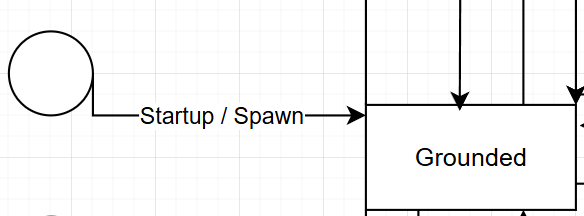
\includegraphics[width=\linewidth]{Diagrams/SpawnIn-Grounded.png}
	\caption{A program elindítása / a karakter újraéledése utáni állapot}
	\label{Spawn_Grounded}
\end{figure}

A karakter mindig egy szilárd, állható talaj fölött éled le, vagy éled újra, ezzel garantálva az állapotok közötti folytonosságot. Az alap állapot minden esetben az ún. "Idle", avagy nyugalmi állapot lesz, ahol a karakter egy állható, szilárd talajon van és játékos nem ad meg bemenetet, ez a \ref{Grounded_Idle} ábrán látható.

\begin{figure}[H]
	\centering
	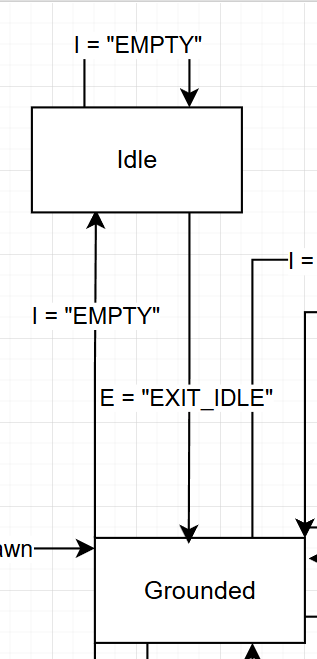
\includegraphics[height = 659px/2, width = 317px/2]{Diagrams/Grounded-Idle.png}
	\caption{A karakter egyhelyben állása}
	\label{Grounded_Idle}
\end{figure}

Ebben az állapotban egy nyugalmi animáció játszódik le, ami életszerűbbé teszi a karaktert. A szilárd talajon való állásból (Grounded) elindulhat a játékos valamely mozgás gomb lenyomásával az egyik irányba ezzel átlökve az automatát a mozgásban levés állapotába (Moving), ahogyan azt a \ref{Grounded_Moving} ábra is mutatja.

\begin{figure}[H]
	\centering
	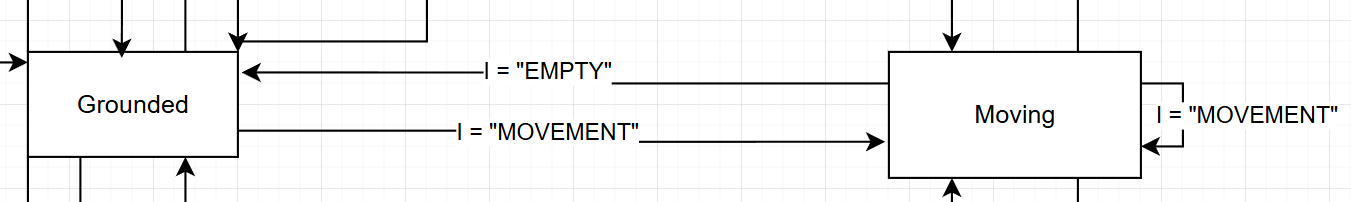
\includegraphics[width=\linewidth]{Diagrams/Grounded-Movement.png}
	\caption{A karakter állható talajon való mozgása}
	\label{Grounded_Moving}
\end{figure}

Ebből az állapotból a játékos visszatérhet a Grounded állapotba ha abba hagyja a mozgást. Viszont, ha a játékos mozgás közben lenyomja az ugrás gombot (ami ebben az esetben a "SPACE"), akkor átlöki az automatát a levegőben lévő állapotba (InAir), ami az alábbi \ref{Moving_InAir} ábrán látható.

\begin{figure}[H]
	\centering
	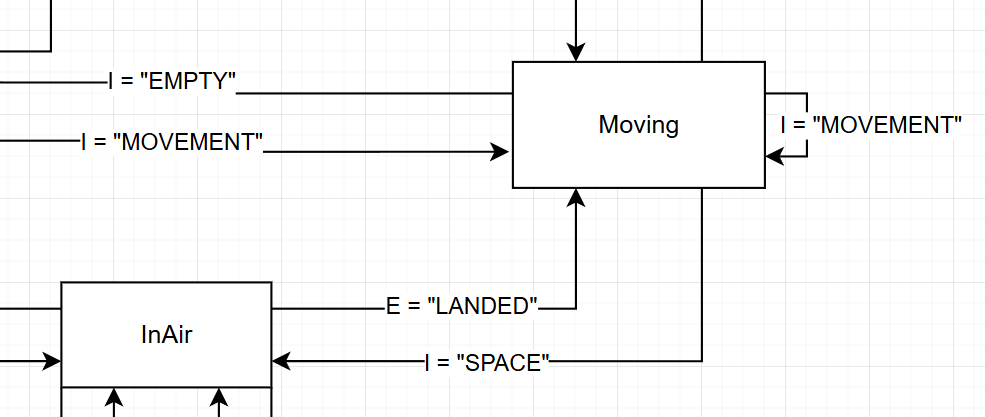
\includegraphics[width=\linewidth]{Diagrams/Moving-InAir.png}
	\caption{A karakter mozgásból való ugrása}
	\label{Moving_InAir}
\end{figure}

Az ugrás időhöz van kötve, amit a gravitációs vonzóerőből és a sebességből számol ki a program. Amint ez az idő lejár és a karakter földet ér a program kiad egy "földet ért" (LANDED) eseményt, amiből, abban az esetben ha a játékos még mindig mozog, akkor visszatér a Moving állapotba. Amennyiben, viszont a játékos már nem ad meg bemenetet a mozgásra, akkor az InAir állapotból visszatérünk a Grounded állapotra, amit a \ref{Grounded_InAir} ábra demonstrál.

\begin{figure}[H]
	\centering
	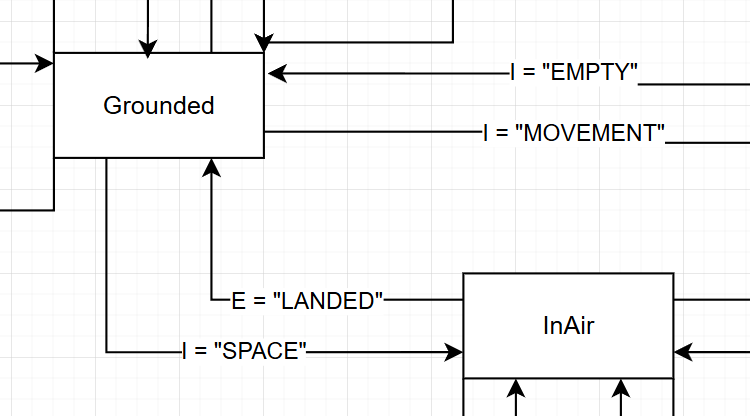
\includegraphics[width=\linewidth]{Diagrams/InAir-Grounded.png}
	\caption{A karakter állható talajról való ugrása}
	\label{Grounded_InAir}
\end{figure}

Vegyük észre, hogy a Grounded állapotból is el lehet jutni az InAir állapotba, abban az esetben, ha a játékos nem ad meg mozgásra bemenetet, viszont ugrásra igen. Ha a játékosnak viszont kell még egy kis idő a levegőben, akkor még egyszer megnyomva az ugrás gombot, akkor átlöki az automatát a dupla ugrás (DoubleJump) állapotba, ahogy azt a \ref{InAir_DoubleJump} ábrán is lehet látni. Ebben az állapotban megtartja a momentumát a játékos csak a felfele mutató vektorhoz adódik hozzá megint az érték.

\begin{figure}[H]
	\centering
	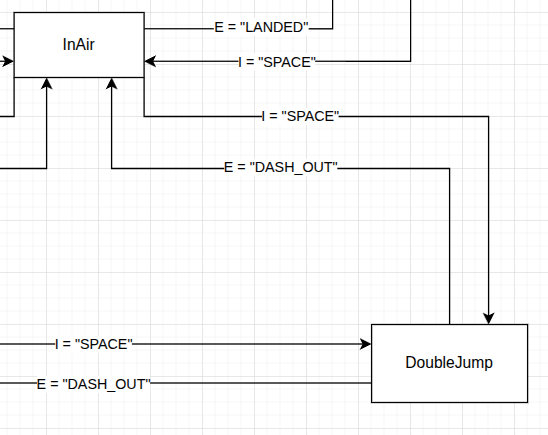
\includegraphics[width=\linewidth]{Diagrams/InAir-DoubleJump.png}
	\caption{A karakter levegőből való ugrása}
	\label{InAir_DoubleJump}
\end{figure}

Vegyük észre, hogy a játékosnak most már nincs irányítása a karakter levegőben maradása fölött, mivel kaptunk egy eseményt, ami megmondta nekünk, hogy nincs több ugrásunk ("DASH\_OUT"). Abban az esetben ha a játékos a dupla ugrás után tovább szeretné mozgatni a karaktert a levegőben valamilyen okból kifolyólag, akkor a mozgás billentyűket lenyomva át tudja lökni az automatát a levegőben lévő mozgás (InAirMovement) állapotba, ahogyan azt a \ref{DoubleJump_InAirMovement} ábra is mutatja. Amíg a játékos lenyomva tartja a mozgás gombokat, addig ebben az állapotban marad.

\begin{figure}[H]
	\centering
	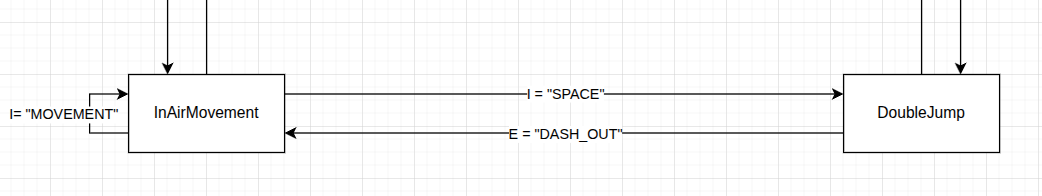
\includegraphics[width=\linewidth]{Diagrams/InAirMovement-DoubleJump.png}
	\caption{A karakter levegőben való mozgása egy dupla ugrás után}
	\label{DoubleJump_InAirMovement}
\end{figure}

Amennyiben a játékos abba hagyja a mozgást, és még nem futott ki a levegőben tölthető időből az automata vissza lesz lökve a levegőbeli állapotba (InAir). Viszont, ha ismét el kezd mozogni, akkor vissza lesz lökve a levegőben lévő mozgás állapotába, ezzel befejezve a kört, ahogy az az alábbi \ref{InAir_InAirMovement} ábrán is látható.

\begin{figure}[H]
	\centering
	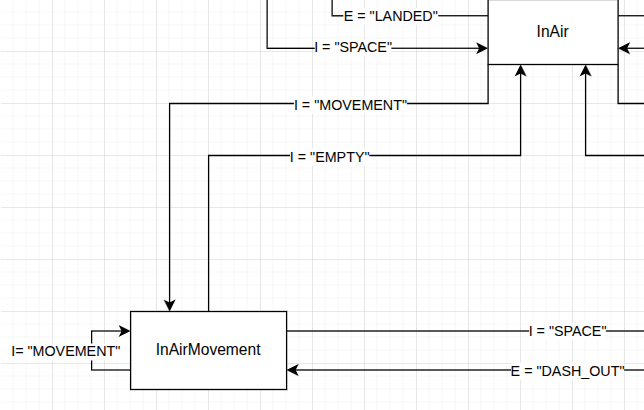
\includegraphics[width=\linewidth]{Diagrams/InAir-InAirMovement.png}
	\caption{A karakter levegőben való mozgása és esésbe való visszatérése}
	\label{InAir_InAirMovement}
\end{figure}

Érdemes megjegyezni, hogy az eddig felsorolt állapotok össze vannak kötve egymással. Ezeket mozgás hármasoknak hívom. A legtöbb mozgásfajtát le lehet bontani kisebb csoportokra amiknek van hozzáférése 1 vagy 2 olyan állapothoz, amely átviszi őket egy másik csoportba.
Példaképpen a levegőben történő mozgáscsoport hármasa a \ref{InAirTrio} ábrán látható.

\begin{figure}[H]
	\centering
	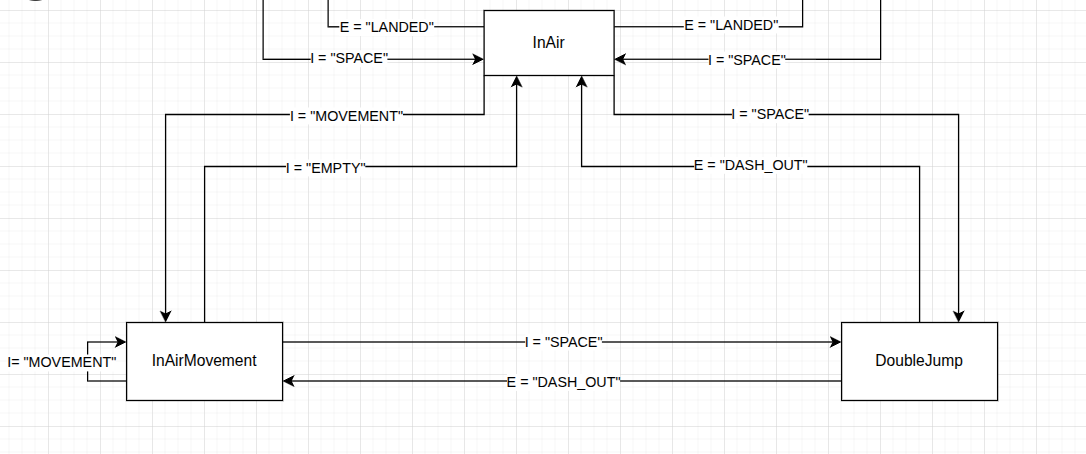
\includegraphics[width=\linewidth]{Diagrams/InAirTrio.png}
	\caption{A levegőben történő mozgáscsoport}
	\label{InAirTrio}
\end{figure}

Valamint a földön történő mozgáscsoport hármasa a \ref{GroundedTrio} ábrán.

\begin{figure}[H]
	\centering
	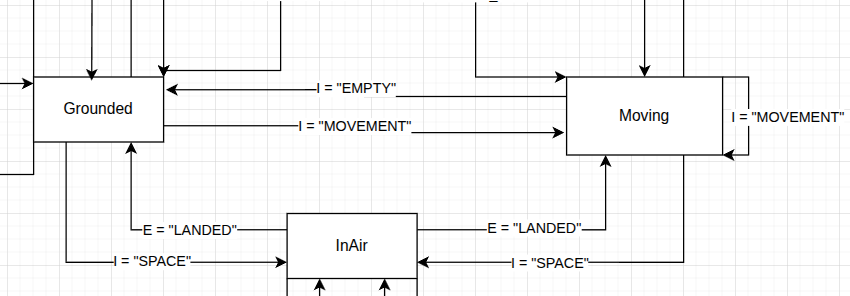
\includegraphics[width=\linewidth]{Diagrams/BaseTrio.png}
	\caption{Az állható talajon történő mozgáscsoport}
	\label{GroundedTrio}
\end{figure}

Ezen mozgáscsoportok közötti átjárást az \textbf{ugrás} cselekvés biztosítja, ami további mozgáslehetőségeket tár fel. Név szerint a dupla ugrás (DoubleJump) és a levegőbeli mozgás (InAirMovement), amikbe a már megszokott "MOVEMENT" cselekvés és "SPACE" gomb lenyomásával tud a felhasználó eljutni.

\subsection{Osztályok}

Az osztályok megtervezéséhez UML osztálydiagrammokat használtam. Első sorban a már \hyperref[subsec:Prog]{\ref{subsec:Prog} alfejezetben} is bemutattot StateMachine és State osztályokat fejlesztettem tovább úgy, hogy jobban illeszkedjenek a mi felhasználásunkhoz.

Kezdve a StateMachine osztállyal, amit átneveztem egy jobban illő "PlayerController" névre. Ahogyan a \ref{PlayerController} ábrán is látható nem változott sokat az előző implementációtól. A módosításokhoz tartozik egy "ui" nevű Control típusú változó, amely a Godot-n belül egy Node, ami a kétdimenziós felületeket veszi maga alá, ebben az esetben arra kell, hogy egy felhasználói felületet alkosson, amin követni tudjuk a jelenlegi állapotokat, valamint egy új Dictionary "elements" néven, a megjeleítéshez szükséges CheckBox Node-ok referenciáit tárolja. Ezeken kívül három metódus lett még hozzáadva: az OnTransitionTo, OnSetMovementState és az OnSetMovementDirection. Ezek mind a Player osztályból jövő jelek (Signal) fogadására vannak.

\begin{figure}[H]
	\centering
	 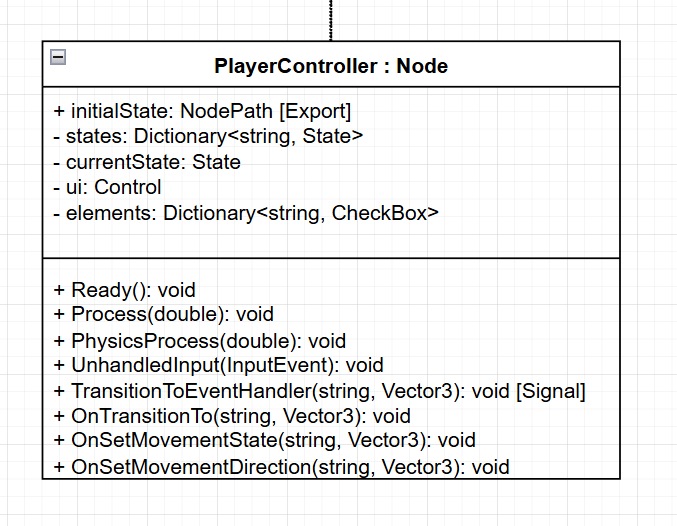
\includegraphics[width=\linewidth]{Diagrams/PlayerController.png}
	\caption{A PlayerController osztálydiagramja}
	\label{PlayerController}
\end{figure}

A State osztály még kevesebbet változott. Ahogy a \ref{State} ábrán is látható három attribútummal bővült az osztály: gravity, parent és movementDirection. A "parent" a játékos Node-ra tart egy referenciát, hogy annak a változóihoz hozzá tudjon jutni, ha arra szükség lenne. A "movementDirection" a mozgás kiszámításához tartozik, a gravity, pedig a gravitációs erőnek, ugráskor.

\begin{figure}[H]
	\centering
	 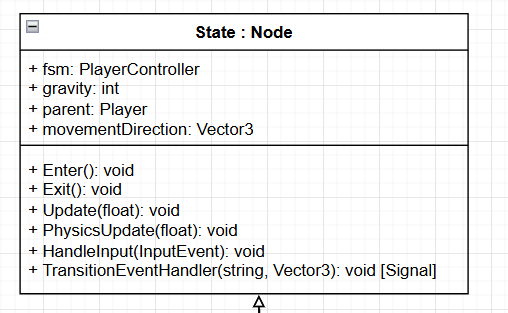
\includegraphics[width=\linewidth]{Diagrams/State.png}
	\caption{A State osztálydiagramja}
	\label{State}
\end{figure}

A Player osztály a játékost írja le. Itt kerül kiszámításra a mozgási irány és a kamera mozgása.  Ahogyan a \ref{Player} ábrán is látható ez egy eléggé nagy osztály, viszont többnyire csak változókkal van tele, amiket az állapotgépünk figyel.  Ezek közül a legfontosabb értékek nekünk a movementDirection, grounded, shapeCast és anim változók.

A movementDirection a játékos mozgási irányának a tárolására van. Ezt  adjuk tovább majd az egyes állapotoknak. A grounded változónk tárolja a játékos földön létét. A shapeCast egy ShapeCast3D objektumot tárol. Ezek az objektumok felvesznek egy primitív alakzatot és annak a határvonalait használja ütközésviszgálatra, akármi, ami ezen az alakzaton belül van, azt le lehet kérdezni. Végül az anim változó animációkat tárol a játékos modellünkhöz, ezeket el tudjuk indítani és meg tudjuk állítani.

A PlayerState változónk egy enum, amely a meglévő állapotokat tárolja. Minden frame kirajzolásánál a jelenlegi állapotot, amit a CurrentState válto\-zóban tárolunk, továbbdobjuk a PlayerControllernek, ami ezek után átlökődik abba az állapotba.

\begin{figure}[H]
	\centering
	 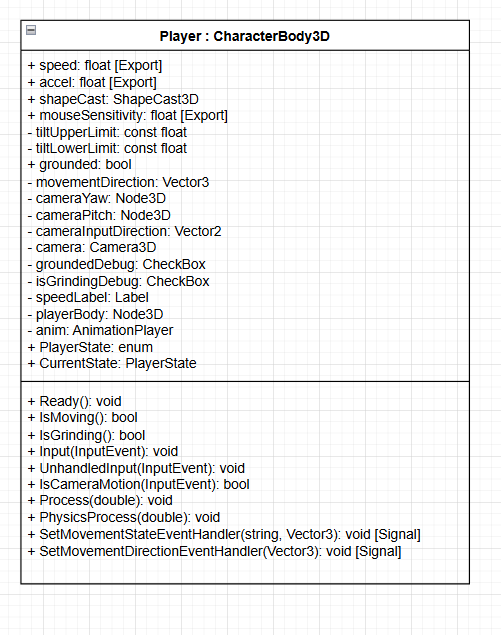
\includegraphics[width=\linewidth]{Diagrams/Player.png}
	\caption{A Player osztálydiagramja}
	\label{Player}
\end{figure}
\newpage

A \ref{Inheritance} ábrán láthatjuk az összes állapotot, amelyet a State osztályból származtatunk le.  A tervezett állapotaink az Idle, a Running, a Jumping, a Falling és a Grinding állapotok, ezekről bővebben beszámolok majd a \hyperref[chap:implementation]{\ref{chap:implementation} fejezetben}.

\begin{figure}[H]
	\centering
	 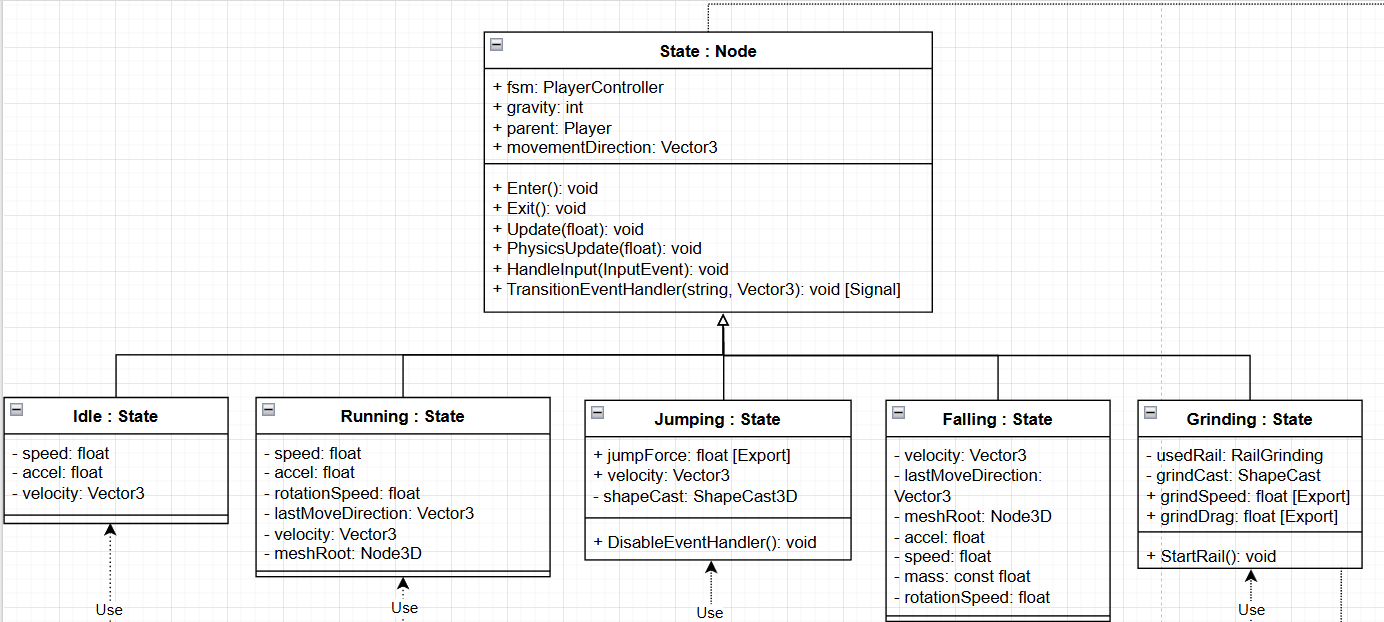
\includegraphics[width=\linewidth]{Diagrams/Inheritance.png}
	\caption{Az állapotok osztálydiagramja}
	\label{Inheritance}
\end{figure}

\begin{minipage}{0.5\textwidth}
	\begin{figure}[H]
		\centering
		 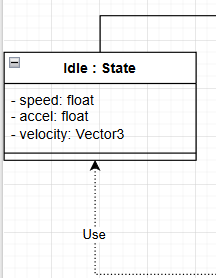
\includegraphics[width=0.9\textwidth]{Diagrams/Idle.png}
		\caption{Az Idle osztálydiagramja}
		\label{Idle}
	\end{figure}
\end{minipage}
\hspace{0.05\textwidth}
\begin{minipage}{0.4\textwidth}
	Ahogy a \ref{Idle} ábrán is látható Idle állapot a karakter egyhelyben állásáért felelős és kiegészül egy speed, accel és velocity változóval.
\end{minipage}
\vspace{1cm}

\begin{minipage}{0.4\textwidth}
	A \ref{Running} ábrán látható Running állapot a karakter mozgásáért felelős állapot. A már említett speed, accel és velocity változókon kívül kiegészül még egy rotationSpeed, lastMoveDirection és meshRoot változókkal. A lastMoveDirection, rotationSpeed és meshRoot változók a modell forgatásához kell, hogy ugyan abba az irányba nézzen, amelybe megy.
\end{minipage}
\hspace{0.05\textwidth}
\begin{minipage}{0.5\textwidth}
	\begin{figure}[H]
		\centering
		 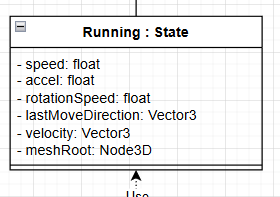
\includegraphics[width=\textwidth]{Diagrams/Running.png}
		\caption{A Running osztálydiagramja}
		\label{Running}
	\end{figure}
\end{minipage}
\vspace{1cm}

\begin{minipage}{0.5\textwidth}
	\begin{figure}[H]
		\centering
		 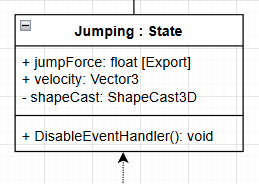
\includegraphics[width=0.9\textwidth]{Diagrams/Jumping.png}
		\caption{A Jumping osztálydiagramja}
		\label{Jumping}
	\end{figure}
\end{minipage}
\hspace{0.05\textwidth}
\begin{minipage}{0.4\textwidth}
	A \ref{Jumping} ábrán Jumping állapot a karakter ugrásáért felelős. Kiegészül a jumpForce, velocity és shapeCast változókkal és DisableEventHandler metódussal. Az ugráshoz fontos jumpForce befolyásolja, hogy milyen erővel rugaszkodik el a karakter a földtől.
\end{minipage}
\vspace{1cm}

\begin{minipage}{0.4\textwidth}
	A \ref{Falling} ábrán látható Falling állapot az ugrást követő esésnek a lebonyolítására szolgál, valamint ügyel arra, hogy a levegőben töltött idő közben a játékosnak legyen egy kis irányítása a karakter felett. Kiegészül az eséshez szükséges mass változóval, a mozgáshoz szükséges: velocity, accel és speed változókkal. Valamint a forgáshoz szükséges: meshRoot, rotationSpeed és lastMoveDirection változókkal.
\end{minipage}
\hspace{0.05\textwidth}
\begin{minipage}{0.5\textwidth}
	\begin{figure}[H]
		\centering
		 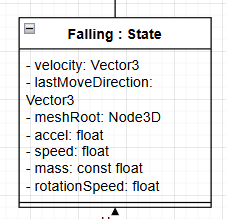
\includegraphics[width=\textwidth]{Diagrams/Falling.png}
		\caption{A Falling osztálydiagramja}
		\label{Falling}
	\end{figure}
\end{minipage}
\vspace{1cm}

\begin{minipage}{0.5\textwidth}
	\begin{figure}[H]
		\centering
		 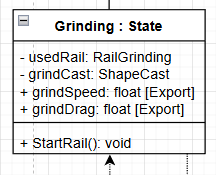
\includegraphics[width=0.9\textwidth]{Diagrams/Grinding.png}
		\caption{A Grinding osztálydiagramja}
		\label{Grinding}
	\end{figure}
\end{minipage}
\hspace{0.05\textwidth}
\begin{minipage}{0.4\textwidth}
	A \ref{Grinding} ábrán látható Grinding állapot felelős a csúszásért különböző erre alkalmas felületeken. Kiegészül egy usedRail, grindCast, grindSpeed és grindDrag változókkal, és a StartRail metódussal. Érdemes megjegyezni, hogy a usedRail RailGrinding típusú, tehát függősége lesz a Grinding osztálynak a RailGrinding osztály, ahogy azt a \ref{RailGrinding-Grinding} ábra is mutatja.
\end{minipage}
\vspace{1cm}

A \ref{RailGrinding-Grinding} ábrán szintúgy látható RailGrinding osztály maguknak a csúszásra alkalmas objektumoknak a vezérlését felügyelik. Rendelkezik egy path és egy pathFollow változóval, valamint a Ready és CalculateTargetRailPoint metódusokkal. A path változó magát az utat tárolja, amit a játékos csúszás közben követni fog és a pathFollow ennek az útnak a pontjait tárolja.

\begin{figure}[H]
	\centering
	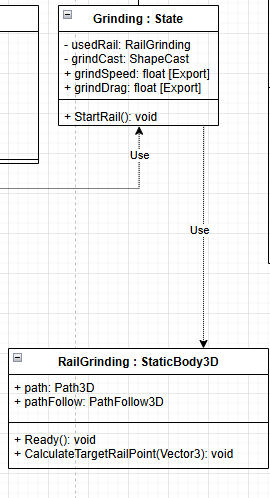
\includegraphics[height=489px , width=270px]{Diagrams/Grinding-RailGrinding.png}
	\caption{A Grinding és RailGrinding közötti kapcsolat}
	\label{RailGrinding-Grinding}
\end{figure}

A \ref{StateUse} ábra mutatja a PlayerController és a többi állapot közötti kap\-csolatot. A PlayerController felhasználja az egyes állapotok metódusait, ezért függőség alakul ki köztük. Amikor az állapotgéphez hozzáadunk egy új állapotot ez a függőség egyből létrejön.

\begin{figure}[h]
	\centering
	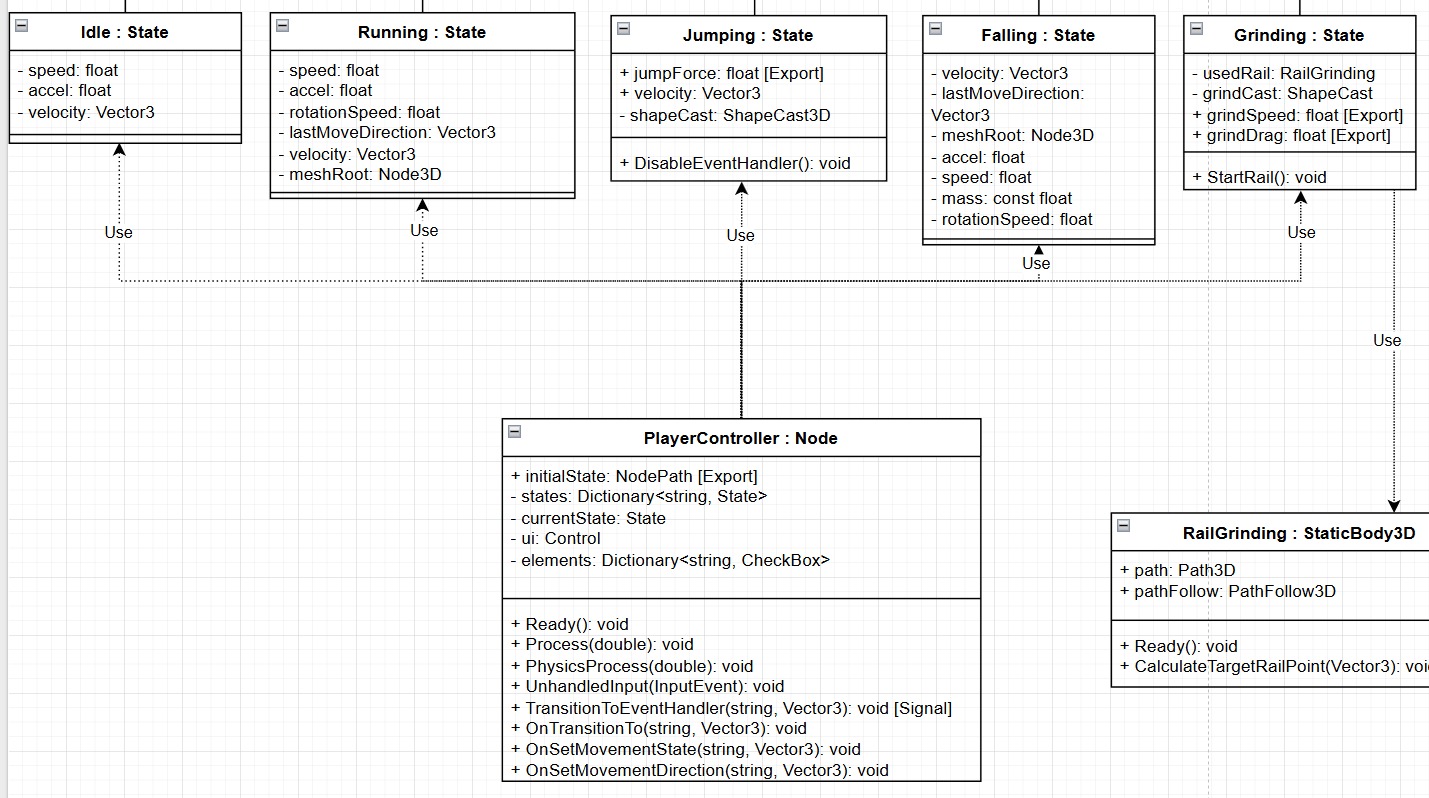
\includegraphics[height=0.8\linewidth , angle=-90]{Diagrams/StateUses.png}
	\caption{A PlayerController és a többi állapot kapcsolata}
	\label{StateUse}
\end{figure}
